% =====================================================================
%  PeakCheck — Anleitung (Deutsch)
%  Kompilieren: pdflatex Anleitung_PeakCheck.tex  (2x für Verweise)
% =====================================================================
\documentclass[11pt,a4paper]{article}
\def\peakchecklang{ngerman}
% =====================================================================
%  PeakCheck — shared LaTeX preamble
%  Used by:  Anleitung_PeakCheck.tex (DE), Manual_PeakCheck_EN.tex (EN),
%            Supplement_PeakCheck_EN.tex (EN)
%
%  Set the document language BEFORE % =====================================================================
%  PeakCheck — shared LaTeX preamble
%  Used by:  Anleitung_PeakCheck.tex (DE), Manual_PeakCheck_EN.tex (EN),
%            Supplement_PeakCheck_EN.tex (EN)
%
%  Set the document language BEFORE % =====================================================================
%  PeakCheck — shared LaTeX preamble
%  Used by:  Anleitung_PeakCheck.tex (DE), Manual_PeakCheck_EN.tex (EN),
%            Supplement_PeakCheck_EN.tex (EN)
%
%  Set the document language BEFORE \input{preamble.tex}, e.g.
%      \def\peakchecklang{english}   % or:  \def\peakchecklang{ngerman}
%  Engine: pdflatex.  Bibliography: bibtex + natbib (plainnat).
% =====================================================================

\usepackage[T1]{fontenc}
\usepackage[utf8]{inputenc}
\providecommand{\peakchecklang}{english}
% Graceful fallback: if the requested German babel files are absent (minimal
% TeX Live), fall back to english so the file still compiles. A full TeX Live /
% Overleaf has texlive-lang-german, so there the document stays German.
\def\pklangde{ngerman}
\ifx\peakchecklang\pklangde
  \IfFileExists{ngermanb.ldf}{}{\def\peakchecklang{english}}
\fi
\usepackage[\peakchecklang]{babel}
\IfFileExists{lmodern.sty}{\usepackage{lmodern}}{}

\usepackage[a4paper,margin=2.3cm]{geometry}
\usepackage{amsmath}
\usepackage{amssymb}
\usepackage{mathtools}
\usepackage{graphicx}
\usepackage{xcolor}
\usepackage{listings}
\usepackage{booktabs}
\usepackage{array}
\usepackage{tabularx}
\usepackage{ragged2e}
\usepackage{enumitem}
\usepackage{caption}
\usepackage[numbers,sort&compress]{natbib}
\IfFileExists{microtype.sty}{\usepackage[protrusion=true,expansion=false]{microtype}}{}

% hyperref last
\usepackage[colorlinks=true,linkcolor=pkblue,citecolor=pkblue,urlcolor=pkblue]{hyperref}

% --- colours ---------------------------------------------------------
\definecolor{pkblue}{HTML}{1F4E79}
\definecolor{pkaccent}{HTML}{C55A11}
\definecolor{codebg}{HTML}{F4F6F8}
\definecolor{codeframe}{HTML}{D6DEE6}
\definecolor{kw}{HTML}{0B5394}
\definecolor{str}{HTML}{7F6000}
\definecolor{cmt}{HTML}{6A737D}
\definecolor{hdrgray}{HTML}{555555}

% --- captions --------------------------------------------------------
\captionsetup{font=small,labelfont=bf,labelsep=period}

% --- listings: Python -----------------------------------------------
\lstdefinestyle{py}{%
  language=Python,
  basicstyle=\ttfamily\footnotesize,
  keywordstyle=\color{kw}\bfseries,
  stringstyle=\color{str},
  commentstyle=\color{cmt}\itshape,
  numberstyle=\tiny\color{cmt},
  backgroundcolor=\color{codebg},
  frame=single,
  framerule=0.4pt,
  rulecolor=\color{codeframe},
  showstringspaces=false,
  breaklines=true,
  breakatwhitespace=true,
  columns=fullflexible,
  keepspaces=true,
  tabsize=4,
  xleftmargin=10pt,
  xrightmargin=4pt,
  aboveskip=2pt,
  belowskip=10pt,
}

% --- listings: TOML / console (generic, '#' comments) ---------------
\lstdefinestyle{conf}{%
  basicstyle=\ttfamily\footnotesize,
  keywordstyle=\color{kw},
  commentstyle=\color{cmt}\itshape,
  morecomment=[l]{\#},
  morestring=[b]",
  stringstyle=\color{str},
  backgroundcolor=\color{codebg},
  frame=single,
  framerule=0.4pt,
  rulecolor=\color{codeframe},
  showstringspaces=false,
  breaklines=true,
  columns=fullflexible,
  keepspaces=true,
  xleftmargin=10pt,
  xrightmargin=4pt,
  aboveskip=2pt,
  belowskip=10pt,
}

% --- helper macros ---------------------------------------------------
% inline monospace (detokenize so _, #, & etc. need no escaping)
\newcommand{\code}[1]{\texttt{\detokenize{#1}}}
% header line shown above a code listing: module path + function
\newcommand{\codehdr}[1]{\par\smallskip\noindent
  {\small\ttfamily\color{hdrgray}#1}\par\nobreak\vspace{1pt}}
% a "source / code reference" margin-style note inline
\newcommand{\srcref}[1]{\textnormal{\small\color{hdrgray}(#1)}}

% nicer default spacing for itemize
\setlist[itemize]{leftmargin=1.4em,topsep=2pt,itemsep=1pt}
\setlist[enumerate]{leftmargin=1.6em,topsep=2pt,itemsep=2pt}

% table helpers
\newcolumntype{L}{>{\RaggedRight\arraybackslash}X}
\renewcommand{\arraystretch}{1.15}

% section formatting (lightweight; optional package)
\IfFileExists{sectsty.sty}{\usepackage{sectsty}\allsectionsfont{\color{pkblue}}}{}

\setlength{\parskip}{0.4em}
\setlength{\parindent}{0pt}
, e.g.
%      \def\peakchecklang{english}   % or:  \def\peakchecklang{ngerman}
%  Engine: pdflatex.  Bibliography: bibtex + natbib (plainnat).
% =====================================================================

\usepackage[T1]{fontenc}
\usepackage[utf8]{inputenc}
\providecommand{\peakchecklang}{english}
% Graceful fallback: if the requested German babel files are absent (minimal
% TeX Live), fall back to english so the file still compiles. A full TeX Live /
% Overleaf has texlive-lang-german, so there the document stays German.
\def\pklangde{ngerman}
\ifx\peakchecklang\pklangde
  \IfFileExists{ngermanb.ldf}{}{\def\peakchecklang{english}}
\fi
\usepackage[\peakchecklang]{babel}
\IfFileExists{lmodern.sty}{\usepackage{lmodern}}{}

\usepackage[a4paper,margin=2.3cm]{geometry}
\usepackage{amsmath}
\usepackage{amssymb}
\usepackage{mathtools}
\usepackage{graphicx}
\usepackage{xcolor}
\usepackage{listings}
\usepackage{booktabs}
\usepackage{array}
\usepackage{tabularx}
\usepackage{ragged2e}
\usepackage{enumitem}
\usepackage{caption}
\usepackage[numbers,sort&compress]{natbib}
\IfFileExists{microtype.sty}{\usepackage[protrusion=true,expansion=false]{microtype}}{}

% hyperref last
\usepackage[colorlinks=true,linkcolor=pkblue,citecolor=pkblue,urlcolor=pkblue]{hyperref}

% --- colours ---------------------------------------------------------
\definecolor{pkblue}{HTML}{1F4E79}
\definecolor{pkaccent}{HTML}{C55A11}
\definecolor{codebg}{HTML}{F4F6F8}
\definecolor{codeframe}{HTML}{D6DEE6}
\definecolor{kw}{HTML}{0B5394}
\definecolor{str}{HTML}{7F6000}
\definecolor{cmt}{HTML}{6A737D}
\definecolor{hdrgray}{HTML}{555555}

% --- captions --------------------------------------------------------
\captionsetup{font=small,labelfont=bf,labelsep=period}

% --- listings: Python -----------------------------------------------
\lstdefinestyle{py}{%
  language=Python,
  basicstyle=\ttfamily\footnotesize,
  keywordstyle=\color{kw}\bfseries,
  stringstyle=\color{str},
  commentstyle=\color{cmt}\itshape,
  numberstyle=\tiny\color{cmt},
  backgroundcolor=\color{codebg},
  frame=single,
  framerule=0.4pt,
  rulecolor=\color{codeframe},
  showstringspaces=false,
  breaklines=true,
  breakatwhitespace=true,
  columns=fullflexible,
  keepspaces=true,
  tabsize=4,
  xleftmargin=10pt,
  xrightmargin=4pt,
  aboveskip=2pt,
  belowskip=10pt,
}

% --- listings: TOML / console (generic, '#' comments) ---------------
\lstdefinestyle{conf}{%
  basicstyle=\ttfamily\footnotesize,
  keywordstyle=\color{kw},
  commentstyle=\color{cmt}\itshape,
  morecomment=[l]{\#},
  morestring=[b]",
  stringstyle=\color{str},
  backgroundcolor=\color{codebg},
  frame=single,
  framerule=0.4pt,
  rulecolor=\color{codeframe},
  showstringspaces=false,
  breaklines=true,
  columns=fullflexible,
  keepspaces=true,
  xleftmargin=10pt,
  xrightmargin=4pt,
  aboveskip=2pt,
  belowskip=10pt,
}

% --- helper macros ---------------------------------------------------
% inline monospace (detokenize so _, #, & etc. need no escaping)
\newcommand{\code}[1]{\texttt{\detokenize{#1}}}
% header line shown above a code listing: module path + function
\newcommand{\codehdr}[1]{\par\smallskip\noindent
  {\small\ttfamily\color{hdrgray}#1}\par\nobreak\vspace{1pt}}
% a "source / code reference" margin-style note inline
\newcommand{\srcref}[1]{\textnormal{\small\color{hdrgray}(#1)}}

% nicer default spacing for itemize
\setlist[itemize]{leftmargin=1.4em,topsep=2pt,itemsep=1pt}
\setlist[enumerate]{leftmargin=1.6em,topsep=2pt,itemsep=2pt}

% table helpers
\newcolumntype{L}{>{\RaggedRight\arraybackslash}X}
\renewcommand{\arraystretch}{1.15}

% section formatting (lightweight; optional package)
\IfFileExists{sectsty.sty}{\usepackage{sectsty}\allsectionsfont{\color{pkblue}}}{}

\setlength{\parskip}{0.4em}
\setlength{\parindent}{0pt}
, e.g.
%      \def\peakchecklang{english}   % or:  \def\peakchecklang{ngerman}
%  Engine: pdflatex.  Bibliography: bibtex + natbib (plainnat).
% =====================================================================

\usepackage[T1]{fontenc}
\usepackage[utf8]{inputenc}
\providecommand{\peakchecklang}{english}
% Graceful fallback: if the requested German babel files are absent (minimal
% TeX Live), fall back to english so the file still compiles. A full TeX Live /
% Overleaf has texlive-lang-german, so there the document stays German.
\def\pklangde{ngerman}
\ifx\peakchecklang\pklangde
  \IfFileExists{ngermanb.ldf}{}{\def\peakchecklang{english}}
\fi
\usepackage[\peakchecklang]{babel}
\IfFileExists{lmodern.sty}{\usepackage{lmodern}}{}

\usepackage[a4paper,margin=2.3cm]{geometry}
\usepackage{amsmath}
\usepackage{amssymb}
\usepackage{mathtools}
\usepackage{graphicx}
\usepackage{xcolor}
\usepackage{listings}
\usepackage{booktabs}
\usepackage{array}
\usepackage{tabularx}
\usepackage{ragged2e}
\usepackage{enumitem}
\usepackage{caption}
\usepackage[numbers,sort&compress]{natbib}
\IfFileExists{microtype.sty}{\usepackage[protrusion=true,expansion=false]{microtype}}{}

% hyperref last
\usepackage[colorlinks=true,linkcolor=pkblue,citecolor=pkblue,urlcolor=pkblue]{hyperref}

% --- colours ---------------------------------------------------------
\definecolor{pkblue}{HTML}{1F4E79}
\definecolor{pkaccent}{HTML}{C55A11}
\definecolor{codebg}{HTML}{F4F6F8}
\definecolor{codeframe}{HTML}{D6DEE6}
\definecolor{kw}{HTML}{0B5394}
\definecolor{str}{HTML}{7F6000}
\definecolor{cmt}{HTML}{6A737D}
\definecolor{hdrgray}{HTML}{555555}

% --- captions --------------------------------------------------------
\captionsetup{font=small,labelfont=bf,labelsep=period}

% --- listings: Python -----------------------------------------------
\lstdefinestyle{py}{%
  language=Python,
  basicstyle=\ttfamily\footnotesize,
  keywordstyle=\color{kw}\bfseries,
  stringstyle=\color{str},
  commentstyle=\color{cmt}\itshape,
  numberstyle=\tiny\color{cmt},
  backgroundcolor=\color{codebg},
  frame=single,
  framerule=0.4pt,
  rulecolor=\color{codeframe},
  showstringspaces=false,
  breaklines=true,
  breakatwhitespace=true,
  columns=fullflexible,
  keepspaces=true,
  tabsize=4,
  xleftmargin=10pt,
  xrightmargin=4pt,
  aboveskip=2pt,
  belowskip=10pt,
}

% --- listings: TOML / console (generic, '#' comments) ---------------
\lstdefinestyle{conf}{%
  basicstyle=\ttfamily\footnotesize,
  keywordstyle=\color{kw},
  commentstyle=\color{cmt}\itshape,
  morecomment=[l]{\#},
  morestring=[b]",
  stringstyle=\color{str},
  backgroundcolor=\color{codebg},
  frame=single,
  framerule=0.4pt,
  rulecolor=\color{codeframe},
  showstringspaces=false,
  breaklines=true,
  columns=fullflexible,
  keepspaces=true,
  xleftmargin=10pt,
  xrightmargin=4pt,
  aboveskip=2pt,
  belowskip=10pt,
}

% --- helper macros ---------------------------------------------------
% inline monospace (detokenize so _, #, & etc. need no escaping)
\newcommand{\code}[1]{\texttt{\detokenize{#1}}}
% header line shown above a code listing: module path + function
\newcommand{\codehdr}[1]{\par\smallskip\noindent
  {\small\ttfamily\color{hdrgray}#1}\par\nobreak\vspace{1pt}}
% a "source / code reference" margin-style note inline
\newcommand{\srcref}[1]{\textnormal{\small\color{hdrgray}(#1)}}

% nicer default spacing for itemize
\setlist[itemize]{leftmargin=1.4em,topsep=2pt,itemsep=1pt}
\setlist[enumerate]{leftmargin=1.6em,topsep=2pt,itemsep=2pt}

% table helpers
\newcolumntype{L}{>{\RaggedRight\arraybackslash}X}
\renewcommand{\arraystretch}{1.15}

% section formatting (lightweight; optional package)
\IfFileExists{sectsty.sty}{\usepackage{sectsty}\allsectionsfont{\color{pkblue}}}{}

\setlength{\parskip}{0.4em}
\setlength{\parindent}{0pt}


\title{\vspace{-1.5em}\color{pkblue}\bfseries PeakCheck --- Anleitung\\[2pt]
\normalsize\mdseries\color{black}Interaktives Multipeak-Fitting und
Peak-Pr\"asenz-Pr\"ufung f\"ur beliebige x/y-Daten}
\author{Lukas Knauer\\[-2pt]
{\small RPTU Kaiserslautern-Landau \textperiodcentered\ AG Sch\"unemann}}
\date{\small Version 1.0.0 \textperiodcentered\ MIT-Lizenz \textperiodcentered\ 2026}

\hypersetup{
  pdftitle={PeakCheck -- Anleitung},
  pdfauthor={Lukas Knauer},
  pdfsubject={PeakCheck Benutzerhandbuch: interaktives Multipeak-Voigt-Fitting und Peak-Praesenz-Pruefung},
  pdfkeywords={Voigt, Peak-Fit, Spektroskopie, PeakCheck}
}

\begin{document}
\maketitle
\thispagestyle{empty}

\noindent\fcolorbox{codeframe}{codebg}{%
\parbox{\dimexpr\linewidth-2\fboxsep\relax}{\small
\textbf{Was macht PeakCheck?} Es bestimmt Peaks in einem Referenzdatensatz (z.\,B.\
einem aufsummierten Spektrum) und pr\"uft anschlie\ss end, ob dieselben Peaks in
einem oder mehreren Komponenten-Datens\"atzen (z.\,B.\ Subspektren) vorhanden
sind. Es funktioniert mit beliebigen 2- oder 3-spaltigen x/y-Daten --- Spektren,
Beugungsmuster, Chromatogramme, Messreihen.}}

\begin{figure}[h]
\centering
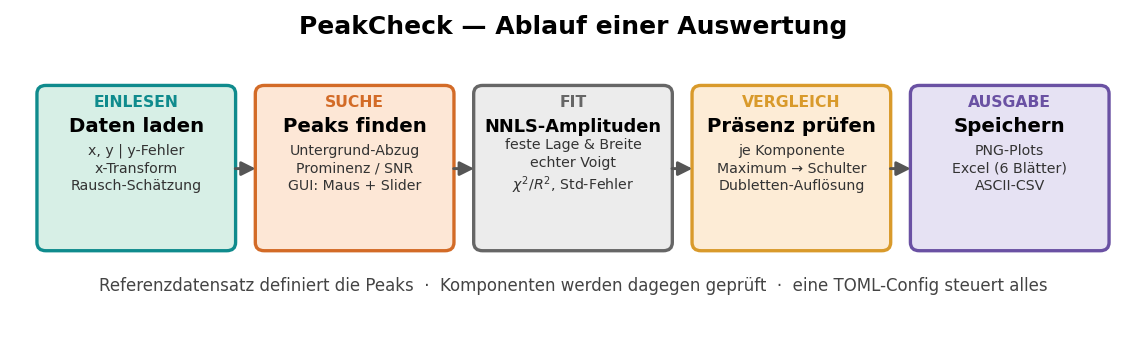
\includegraphics[width=0.88\linewidth]{figures/fig_pipeline_de.png}
\caption{Ablauf einer Auswertung: vom Einlesen \"uber Suche und Fit bis zum
Vergleich und zur Ausgabe.}
\end{figure}

% =====================================================================
\section{Installation \& Start}
PeakCheck ist ein kleines Python-Paket mit einem r\"uckw\"artskompatiblen
Starter (\code{peakcheck.py}). Ben\"otigt werden Python 3.10+ sowie die Pakete
\code{numpy}, \code{scipy}, \code{matplotlib}, \code{openpyxl} und Tk f\"ur die
grafische Oberfl\"ache.

\begin{lstlisting}[style=conf]
# Pakete installieren (einmalig)
pip install numpy scipy matplotlib openpyxl
# Tk ist bei Windows/macOS schon dabei; unter Linux:
sudo apt install python3-tk
# Fuer Python < 3.11 zusaetzlich der TOML-Leser:
pip install tomli
\end{lstlisting}

Es gibt drei gleichwertige Wege, das Programm zu starten --- nimm den, der zu
deiner Arbeitsweise passt:

\begin{lstlisting}[style=conf]
# 1) Grafisch (Standard): Fenster oeffnen, einstellen, klicken, fitten
python -m peakcheck            # oder einfach: peakcheck   (nach pip install)
python peakcheck.py            # funktioniert weiterhin als Starter

# 2) Ohne Fenster, gesteuert ueber eine TOML-Datei (Batch/HPC)
python -m peakcheck --config job.toml --no-gui

# 3) Eine kommentierte Konfigurationsvorlage schreiben
python -m peakcheck --write-template job.toml
\end{lstlisting}

\noindent\textit{In Spyder am besten als eigenst\"andiges Programm starten (nicht
in der IPython-Konsole), damit sich ein echtes Fenster \"offnet. Alternativ in der
Konsole vorher \code{\%matplotlib qt5} setzen.}

% =====================================================================
\section{Eingabedaten}
PeakCheck liest spaltenweise Textdaten unabh\"angig von der Dateiendung:
\code{.dat}, \code{.txt}, \code{.csv}, \code{.xy}, \code{.asc}, \code{.tsv},
\code{.prn}, \code{.nis} und \"ahnliche funktionieren, solange die Datei zwei
oder drei numerische Spalten enth\"alt. Werte d\"urfen durch Leerzeichen,
Tabulatoren, Kommas oder Semikola getrennt sein; Kopfzeilen, Kommentarzeichen
(\code{# ! \%}) und ein deutsches Dezimalkomma (z.\,B.\ \code{10,5}) werden
automatisch erkannt und behandelt. (Einzig \code{.fio} wird gesondert behandelt;
siehe unten.)

\begin{table}[h]\small\centering
\begin{tabularx}{\linewidth}{@{}l l L@{}}
\toprule
\textbf{Format} & \textbf{Bedeutung} & \textbf{Auswirkung auf den Fit}\\
\midrule
\code{x  y} & zwei Spalten, keine Fehler & ungewichteter Fit; Rauschen wird aus den Daten gesch\"atzt\\
\code{x  y  y_fehler} & drei Spalten mit Messfehler & gewichteter Fit; Fehler gehen als $1/\sigma$ in den Fit ein\\
\bottomrule
\end{tabularx}
\end{table}

\noindent\textbf{FIO-Dateien (DESY/PETRA III).} Dateien mit der Endung
\code{.fio} werden direkt gelesen: PeakCheck wertet den \code{\%d}-Datenblock mit
seinen \code{Col}-Spaltendeklarationen aus (die \code{\%c}/\code{\%p}-Kommentar-
und Parameterbl\"ocke werden ignoriert). Da solche Dateien viele Spalten
enthalten, w\"ahlen zwei Einstellungen die gew\"unschten aus:
\code{fio_x_column} (Standard: erste Spalte, meist die Energieachse) und
\code{fio_y_column} (Standard \code{"nisp"}, das NIS-Signal). Beides kann ein
Spalten\emph{name} (z.\,B.\ \code{"nfsp"}) oder ein 1-basierter Index sein.
FIO-Dateien haben keine Fehlerspalte, daher wird das Rauschen gesch\"atzt, sofern
\code{error_column} nicht auf eine bestimmte Spalte zeigt.
\code{<name>_*.<endung>}. Liegt die Referenz also in \code{probe.txt}, werden
\code{probe_01.txt}, \code{probe_42.txt} usw.\ als Komponenten erkannt. Das Muster
ist \"uber \code{component_glob} frei einstellbar.

% =====================================================================
\section{Die grafische Oberfl\"ache}
\begin{figure}[h]
\centering
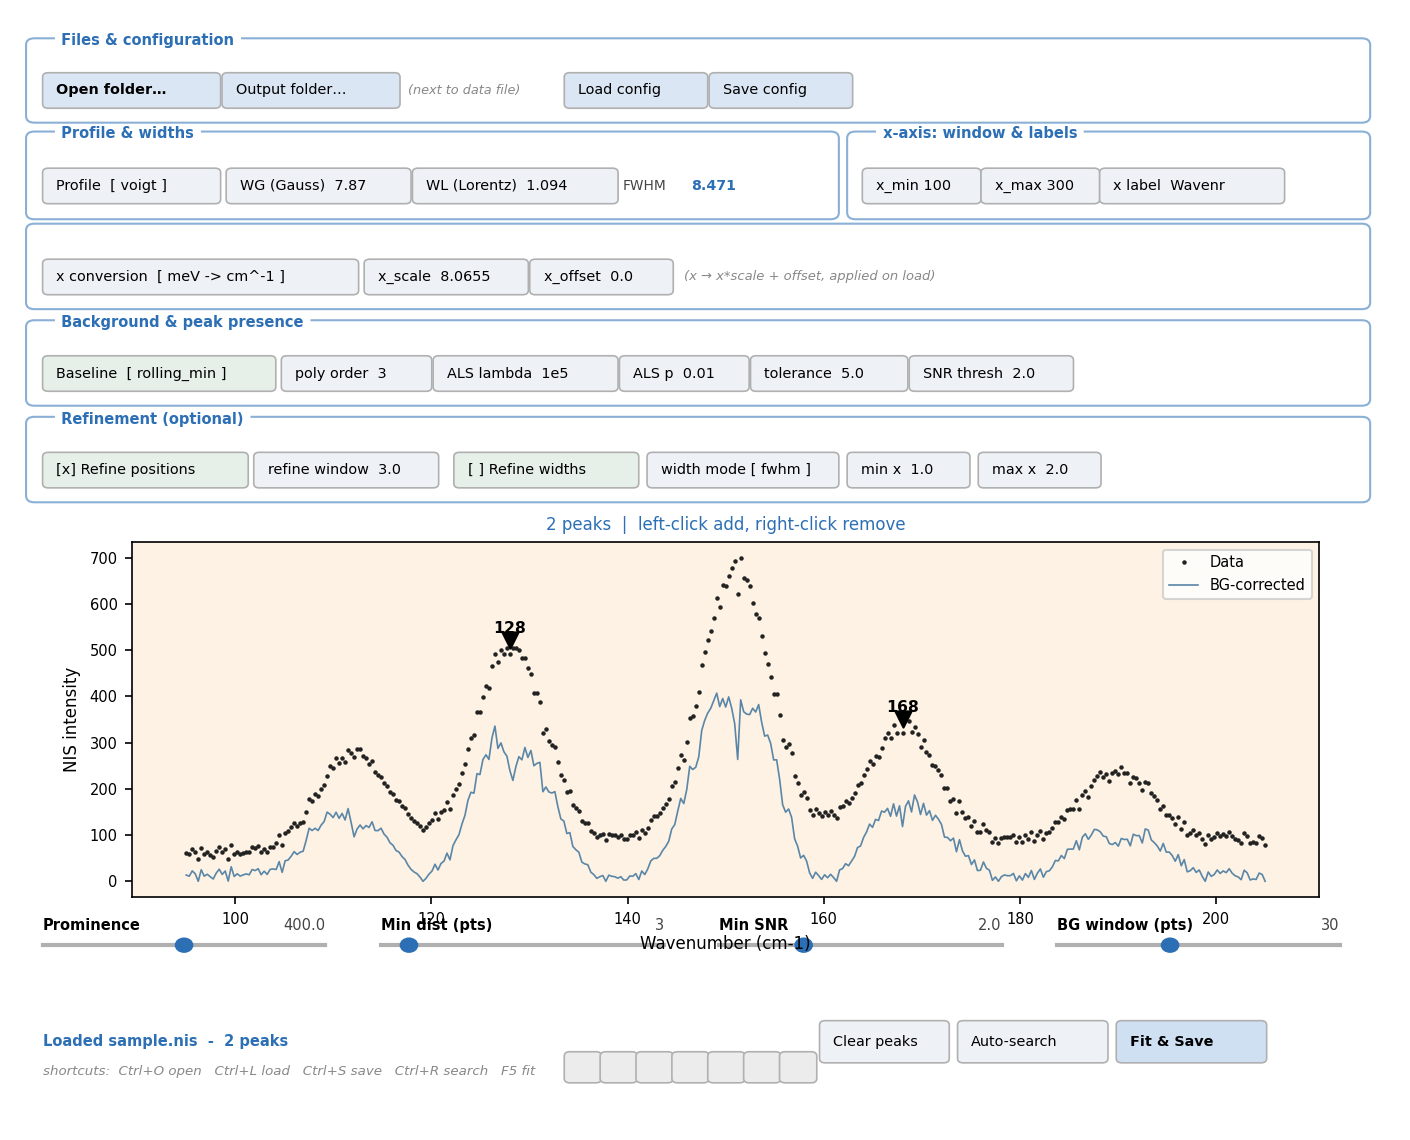
\includegraphics[width=0.92\linewidth]{figures/fig_gui.png}
\caption{Das PeakCheck-Fenster: die Bedienelemente sind in beschriftete Gruppen
gefasst (Dateien \& Konfiguration; Profil \& Breiten; x-Achse: Fenster,
Beschriftungen \& Umrechnung; Untergrund \& Peak-Pr\"asenz; Verfeinerung), gefolgt
vom interaktiven Plot mit Peak-Markern, den Such-Slidern und dem Knopf
\emph{Fit \& Save}. Die Tastaturk\"urzel stehen unten. Felder, die zur aktuellen
Auswahl nicht passen (z.\,B.\ die ALS-Parameter, wenn die Basislinie nicht ALS
ist), sind ausgegraut.}
\label{fig:gui}
\end{figure}

\noindent\textbf{Bedienschritte}
\begin{enumerate}
\item \textbf{Ordner \"offnen} \"uber \emph{Open folder\dots}. Es erscheint ein
Dialog mit allen Datendateien des Ordners. Markiere eine als Referenz
(Radio-Knopf in der Spalte ,,Ref``) und beliebig viele als Komponenten (H\"akchen
in der Spalte ,,Cmp``). Mit \emph{OK} best\"atigen --- die Daten erscheinen sofort
zusammen mit der untergrundkorrigierten Kurve (blau).
\item \textbf{Suchbereich} \"uber \code{x_min}/\code{x_max} eingrenzen (mit
\emph{Enter} best\"atigen); der aktive Bereich wird orange hinterlegt.
\item \textbf{Profil und Breiten} w\"ahlen: \code{voigt}, \code{gauss} oder
\code{lorentz} sowie die Halbwertsbreiten \code{WG} (Gau\ss) und \code{WL}
(Lorentz). Die resultierende effektive FWHM des gew\"ahlten Profils wird daneben
als nicht editierbarer Wert angezeigt (sie aktualisiert sich beim Bearbeiten von
\code{WG}/\code{WL} oder des Profils).
\item \textbf{Peaks finden}: mit den vier Slidern (Prominenz, Mindestabstand,
Mindest-SNR, Untergrundfenster) die automatische Suche steuern; was jeder einzelne
bewirkt, steht unten unter ,,Parameter w\"ahlen \& gute Praxis``.
\item \textbf{Basislinie und Verfeinerung} (vierte Zeile, optional): die
\code{baseline_method} f\"ur den Fit w\"ahlen (\code{rolling_min},
\code{polynomial} oder \code{als}, daneben Polynomgrad und ALS-$\lambda$/$p$) und
\emph{Refine positions} aktivieren, um die Lagen nach dem Fit innerhalb von
\code{refine window} zu verfeinern. Die Standardwerte reproduzieren das bisherige
Verhalten.
\item \textbf{Feinkorrektur per Maus} direkt im Plot:
  \begin{itemize}
  \item \emph{Linksklick} --- f\"ugt am n\"achstgelegenen Datenpunkt einen Peak hinzu
  \item \emph{Rechtsklick} --- entfernt den n\"achstgelegenen Peak-Marker
  \end{itemize}
\item \textbf{Fit \& Save} startet den Fit, die Pr\"asenzpr\"ufung in den
Komponenten und schreibt alle Ausgabedateien.
\end{enumerate}

\noindent\fcolorbox{codeframe}{codebg}{%
\parbox{\dimexpr\linewidth-2\fboxsep\relax}{\small
\textbf{Tipp zur Reihenfolge:} erst den Suchbereich setzen, dann das
Untergrundfenster so justieren, dass die blaue Kurve die Peaks sauber abbildet,
anschlie\ss end Mindest-SNR ($\approx 2$) und Prominenz feinjustieren --- und
zuletzt per Mausklick einzelne Peaks erg\"anzen oder entfernen.}}

\medskip
\noindent \"Uber \emph{Save config} bzw.\ \emph{Load config} lassen sich alle
Einstellungen als TOML-Datei sichern und wieder laden --- so ist jede Auswertung
reproduzierbar.

\subsection{Einheiten der x-Achse umrechnen}
In der dritten Bedienzeile l\"asst sich die x-Achse beim Einlesen umrechnen. Das
Auswahlfeld \emph{x conversion} bietet g\"angige Umrechnungen als Vorlage; sie
setzt \code{x_scale}, \code{x_offset} sowie Achsenbeschriftung und Einheit
automatisch. F\"ur NIS/NRVS w\"ahlst du ,,meV $\to$ cm$^{-1}$`` --- danach l\"auft
die gesamte Auswertung in cm$^{-1}$.

\begin{table}[h]\small\centering
\begin{tabularx}{\linewidth}{@{}l l L@{}}
\toprule
\textbf{Vorlage} & \textbf{Faktor (\code{x_scale})} & \textbf{typische Anwendung}\\
\midrule
meV $\to$ cm$^{-1}$ & 8,065544    & NIS/NRVS, pDOS\\
cm$^{-1}$ $\to$ meV & 0,12398419  & R\"uckrichtung\\
meV $\to$ THz       & 0,24179893  & THz-/inelastische Spektroskopie\\
cm$^{-1}$ $\to$ THz & 0,029979246 & FIR, Phononen\\
eV $\to$ cm$^{-1}$  & 8065,544    & allgemeine Energieachsen\\
meV $\to$ K ($k_B$) & 11,604518   & thermische Skala\\
\bottomrule
\end{tabularx}
\end{table}

Die Umrechnung ist affin ($x \to x\cdot\code{x_scale} + \code{x_offset}$), du
kannst also \"uber die Felder \code{x_scale}/\code{x_offset} auch einen eigenen
Faktor eingeben. Reziproke Umrechnungen wie Wellenl\"ange $\leftrightarrow$
Wellenzahl (cm$^{-1} = 10^{7}/\lambda\,[\mathrm{nm}]$) sind nicht linear und nur
\"uber die TOML-Datei erreichbar (siehe \S4).

\smallskip
\noindent\textit{Wichtig:} Die Umrechnung wird beim Einlesen angewandt. Alle
anderen Werte in x-Einheiten --- \code{x_min}, \code{x_max}, \code{wg},
\code{wl}, \code{tolerance} --- beziehen sich daher auf die bereits umgerechneten
Werte (also z.\,B.\ cm$^{-1}$, nicht meV).

% =====================================================================
\section{Kommandozeile}
Neben der GUI besitzt PeakCheck eine kleine Kommandozeile (das Konsolenskript
\code{peakcheck}, gleichbedeutend \code{python -m peakcheck}):

\begin{table}[h]\small\centering
\begin{tabularx}{\linewidth}{@{}l L@{}}
\toprule
\textbf{Befehl} & \textbf{Wirkung}\\
\midrule
\code{peakcheck} & startet die grafische Oberfl\"ache\\
\code{peakcheck --write-template job.toml} & schreibt eine kommentierte Konfigvorlage und beendet sich\\
\code{peakcheck --config job.toml --no-gui} & l\"auft headless (Batch); ben\"otigt eine Config\\
\code{peakcheck --config job.toml --validate} & pr\"uft eine Config und beendet sich (Exit-Code $\neq 0$ bei Fehler)\\
\code{peakcheck --list-conversions} & listet die x-Achsen-Presets und beendet sich\\
\code{peakcheck --reference data.dat} & \"uberschreibt die Referenzdatei aus der Config\\
\code{peakcheck --output-dir DIR} & schreibt alle Ausgaben nach \code{DIR} (Batch; \"uberschreibt \code{output_dir})\\
\code{peakcheck --version} & gibt die Version aus\\
\code{peakcheck --debug} & zeigt bei Fehlern den vollen Traceback statt einer Kurzmeldung\\
\bottomrule
\end{tabularx}
\end{table}

\noindent Ein Headless-Lauf schreibt exakt dieselben Plots, dieselbe Excel-Mappe und
dieselbe CSV wie die GUI; eine aus der GUI gespeicherte Config reproduziert ihr
Ergebnis also im Batch. \code{--validate} eignet sich in Skripten, um bei einer
fehlerhaften Config sofort abzubrechen. Bei einer fehlerhaften Config oder
Datendatei gibt der Befehl eine kurze \code{PeakCheck: …}-Meldung aus und endet
mit einem Fehlercode; \code{--debug} zeigt den vollen Python-Traceback.

% =====================================================================
\section{Eine erste Analyse}
Das Paket bringt ein lauff\"ahiges Beispiel in \code{example_data/} mit.

\noindent\textbf{Headless, in einer Zeile} (aus \code{example_data/}):
\begin{lstlisting}[style=py]
python -m peakcheck --config nis_example.toml --no-gui
\end{lstlisting}
PeakCheck l\"adt die Referenz \code{sample.nis}, fittet f\"unf Peaks, pr\"uft die
beiden Komponentendateien \code{sample_A.nis} und \code{sample_B.nis} und schreibt
die Plots, die Excel-Mappe und die CSV neben die Daten.

\noindent\textbf{Interaktiv:} \code{peakcheck} starten, \emph{Open folder\dots}
(Strg+O) anklicken und \code{sample.nis} als Referenz, \code{sample_A.nis} und
\code{sample_B.nis} als Komponenten w\"ahlen. Die \emph{x conversion}
\code{meV -> cm^-1} einstellen, \emph{Auto-search peaks} (Strg+R) dr\"ucken oder die
Peaks von Hand anklicken, dann \emph{Fit \& Save} (F5); siehe
Abbildung~\ref{fig:gui}.

\noindent Der Fit reproduziert die Amplituden, $\chi^2_\nu\approx5{,}5$ und
$R^2\approx0{,}945$ aus dem Supplement und meldet, welche der f\"unf Peaks jede
Komponente enth\"alt.

% =====================================================================
\section{Konfiguration \"uber TOML}
F\"ur Batch-L\"aufe und reproduzierbare Pipelines steuert eine TOML-Datei
s\"amtliche Parameter. Eine kommentierte Vorlage erzeugt
\code{python -m peakcheck --write-template job.toml}. Im Folgenden sind alle
verf\"ugbaren Schl\"ussel aufgelistet --- gruppiert nach TOML-Sektion, mit
Standardwert, Beschreibung und Hinweis, wann man sie \"andert.

\paragraph{\code{[input]} --- Eingabe}
\begin{table}[h]\small\centering
\begin{tabularx}{\linewidth}{@{}l l L@{}}
\toprule
\textbf{Schl\"ussel} & \textbf{Default} & \textbf{Bedeutung}\\
\midrule
\code{reference_file} & \code{"data.txt"} & Pfad zur Referenzdatei, in der die Peak-Positionen bestimmt werden. Ein relativer Pfad wird gegen das Verzeichnis der Config-Datei aufgel\"ost, sodass Config und Daten portabel bleiben (batch-tauglich); absolute Pfade werden unver\"andert genutzt. Ein \code{--reference} auf der Kommandozeile \"uberschreibt dies und beh\"alt die \"ubliche Shell-Semantik (relativ zum Arbeitsverzeichnis).\\
\code{component_glob} & \code{""} (leer) & Suchmuster f\"ur Komponentendateien. Leer $=$ automatisch \code{<stem>_*.<ext>} (z.\,B.\ \code{sample.nis} $\to$ \code{sample_A.nis}). Mit explizitem Muster (z.\,B.\ \code{"sub_*.dat"}) \"ubersteuerbar; aus der GUI wird die Auswahl direkt im Ordnerdialog \"ubergeben.\\
\code{error_column} & \code{"auto"} & \code{"auto"} $=$ dritte Spalte als Fehler nutzen, wenn vorhanden, sonst aus den Daten sch\"atzen. \code{"none"} $=$ Fehler immer sch\"atzen. Ganze Zahl $=$ expliziter Spaltenindex (0-basiert).\\
\code{fio_x_column} & \code{""} & nur FIO: x-Spalte per Name oder 1-basiertem Index; leer $=$ erste Spalte.\\
\code{fio_y_column} & \code{"nisp"} & nur FIO: y-Spalte per Name (z.\,B.\ \code{"nfsp"}) oder 1-basiertem Index.\\
\bottomrule
\end{tabularx}
\end{table}

\paragraph{\code{[xaxis]} --- x-Achse}
\begin{table}[h]\small\centering
\begin{tabularx}{\linewidth}{@{}l l L@{}}
\toprule
\textbf{Schl\"ussel} & \textbf{Default} & \textbf{Bedeutung}\\
\midrule
\code{x_conversion} & \code{""} (leer) & Benannte Voreinstellung wie \code{"meV -> cm^-1"}, \code{"cm^-1 -> THz"} oder \code{"nm -> eV (reciprocal)"}. Setzt automatisch Scale, Offset, Beschriftung und Einheit.\\
\code{x_transform} & \code{"affine"} & \code{"affine"}: $x' = x\cdot s + o$ (z.\,B.\ Energieeinheiten). \code{"reciprocal"}: $x' = s/x + o$ (z.\,B.\ Wellenl\"ange $\to$ Wellenzahl).\\
\code{x_scale}, \code{x_offset} & 1.0, 0.0 & Manueller Skalenfaktor und Offset. Wird ignoriert, sobald \code{x_conversion} gesetzt ist.\\
\code{x_label}, \code{y_label} & \code{"x"}, \code{"y"} & Achsenbeschriftungen f\"ur Plots und Ausgabedateien.\\
\code{x_unit} & \code{""} (leer) & Einheit der x-Achse; erscheint in Klammern hinter dem Label und in den Excel-Header-Zeilen (Origin-Stil).\\
\bottomrule
\end{tabularx}
\end{table}

\paragraph{\code{[profile]} --- Linienprofil und Halbwertsbreiten}
\begin{table}[h]\small\centering
\begin{tabularx}{\linewidth}{@{}l l L@{}}
\toprule
\textbf{Schl\"ussel} & \textbf{Default} & \textbf{Bedeutung}\\
\midrule
\code{profile} & \code{"voigt"} & \code{"voigt"} (exakte Faltung Gau\ss$\otimes$Lorentz), \code{"gauss"}, \code{"lorentz"}. Voigt ist der physikalisch korrekte Standard f\"ur die meisten Spektroskopien.\\
\code{wg} & 7.8701 & Gau\ss-FWHM in x-Einheiten --- die instrumentelle Aufl\"osung. Bei NIS an BL09XU (SPring-8): ${\sim}0{,}8$~meV $\approx 6{,}4$~cm$^{-1}$; an P01 (PETRA~III): siehe Beamline-Spezifikation.\\
\code{wl} & 1.094 & Lorentz-FWHM in x-Einheiten --- die nat\"urliche Linienbreite plus thermische Beitr\"age. Bei nicht zerfallenden Phononen \"ublicherweise klein gegen\"uber \code{wg}.\\
\bottomrule
\end{tabularx}
\end{table}

\paragraph{\code{[window]} --- Such- und Fit-Fenster}
\begin{table}[h]\small\centering
\begin{tabularx}{\linewidth}{@{}l l L@{}}
\toprule
\textbf{Schl\"ussel} & \textbf{Default} & \textbf{Bedeutung}\\
\midrule
\code{x_min}, \code{x_max} & \code{""}, \code{""} & Untere und obere Grenze des Auswertungsbereichs in x-Einheiten. Leer $=$ offene Grenze (gesamte Datei). Beeinflusst Peak-Suche und Fit; erscheint zur Identifikation im Dateinamen (z.\,B.\ \code{_100_200}).\\
\code{bg_window} & 30 & Gr\"o\ss e des Fensters f\"ur den Untergrund-Abzug (rollendes Minimum, in Punkten). Faustregel: etwas gr\"o\ss er als ein Peak, deutlich kleiner als die Untergrund-Kr\"ummung. 0 schaltet den Abzug aus.\\
\code{baseline_method} & \code{rolling_min} & Basislinien-Sch\"atzer f\"ur Fit, Statistik und Pr\"asenzpr\"ufung: \code{rolling_min} (Standard), \code{polynomial} oder \code{als} (asymmetrische kleinste Quadrate). Die glatten Varianten eignen sich f\"ur gekr\"ummte Untergr\"unde; \code{baseline_poly_order} (3), \code{baseline_als_lambda} ($10^5$) und \code{baseline_als_p} (0{,}01) stellen sie ein.\\
\bottomrule
\end{tabularx}
\end{table}

\paragraph{\code{[search]} --- Automatische Peak-Suche}
\begin{table}[h]\small\centering
\begin{tabularx}{\linewidth}{@{}l l L@{}}
\toprule
\textbf{Schl\"ussel} & \textbf{Default} & \textbf{Bedeutung}\\
\midrule
\code{prominence_init} & 200.0 & Mindest-Prominenz in y-Einheiten (\code{scipy.signal.find_peaks}). H\"ohere Werte fangen weniger Rauschen, \"ubersehen aber schwache Peaks. In der GUI live per Schieberegler nachstellbar.\\
\code{distance_init} & 3 & Mindestabstand benachbarter Peaks in Punkten. Verhindert, dass eng beieinander liegende Rauschspitzen als zwei Peaks gez\"ahlt werden.\\
\code{min_snr_init} & 2.0 & SNR-Schwelle f\"ur die Auto-Suche (Untergrund-korrigiertes Signal). Erst akzeptiert, wenn die Peak-H\"ohe $\ge \code{min_snr_init}\cdot$Fehler betr\"agt.\\
\bottomrule
\end{tabularx}
\end{table}

\paragraph{\code{[refine]} --- optionale Positions- und Breitenverfeinerung}
Mit \code{refine = true} werden die Peak-Positionen nach dem Fit durch einen
beschr\"ankten nichtlinearen Schritt verfeinert (die Amplituden bleiben
nichtnegativ); \code{refine_window} (Standard 3{,}0, in x-Einheiten) begrenzt, wie
weit sich jede Position verschieben darf. Mit \code{refine_widths = true} wird
zus\"atzlich eine Breite pro Peak verfeinert: \code{width_mode} w\"ahlt, was sich
verbreitert (\code{"fwhm"}, Standard, skaliert den ganzen Voigt; \code{"sigma"}
skaliert nur den Gau\ss-Anteil), und die Breite bleibt zwischen
\code{width_min_factor} und \code{width_max_factor} mal der instrumentellen Breite
(Standard 1{,}0\,..\,2{,}0, also nie schmaler als das Instrument und h\"ochstens
doppelt so breit). Beides ist standardm\"a\ss ig aus; das Ergebnis \"andert sich
also nur, wenn man es aktiviert.

\paragraph{\code{[presence]} --- Pr\"asenzpr\"ufung in den Komponenten}
\begin{table}[h]\small\centering
\begin{tabularx}{\linewidth}{@{}l l L@{}}
\toprule
\textbf{Schl\"ussel} & \textbf{Default} & \textbf{Bedeutung}\\
\midrule
\code{tolerance} & 5.0 & $\pm$ Positionsfenster in x-Einheiten, in dem ein Komponenten-Peak als ,,dasselbe`` wie ein Referenz-Peak gilt. Sollte gr\"o\ss er sein als die typische Schwerpunktsverschiebung zwischen Spektren, kleiner als der Peak-Abstand.\\
\code{snr_thresh} & 2.0 & SNR-Schwelle, ab der ein Peak in der Komponente als ,,vorhanden`` gilt. Bei verrauschten Spektren erh\"ohen (4--6), bei sehr sauberen absenken (2--3).\\
\code{presence_baseline_corrected} & \code{true} & \code{true} $=$ SNR am Untergrund-korrigierten Signal (H\"ohe \"uber Basislinie --- der physikalisch sinnvolle Wert). \code{false} $=$ SNR auf den Rohdaten (enth\"alt Untergrund); selten gew\"unscht.\\
\bottomrule
\end{tabularx}
\end{table}

\paragraph{\code{[errors]} --- Fehlerberichterstattung}
\begin{table}[h]\small\centering
\begin{tabularx}{\linewidth}{@{}l l L@{}}
\toprule
\textbf{Schl\"ussel} & \textbf{Default} & \textbf{Bedeutung}\\
\midrule
\code{error_mode} & \code{"statistical"} & \code{"statistical"} $=$ wahre $1\sigma$ aus $(B^{\top}W^2B)^{-1}$, unskaliert (entspricht \code{absolute_sigma=True} in \code{scipy.curve_fit}). \code{"scaled"} $=$ mit $\sqrt{\chi^2_\mathrm{red}}$ multipliziert --- geeignet, wenn nur relative Fehlergewichtungen bekannt sind.\\
\bottomrule
\end{tabularx}
\end{table}

\paragraph{\code{[output]} --- Ausgabe}
\begin{table}[h]\small\centering
\begin{tabularx}{\linewidth}{@{}l l L@{}}
\toprule
\textbf{Schl\"ussel} & \textbf{Default} & \textbf{Bedeutung}\\
\midrule
\code{output_dir} & \code{""} (leer) & Zielordner f\"ur alle Ausgaben (Plots, Excel, CSV). Leer $=$ neben der Referenzdatei. In der GUI auch per Knopf ,,Output folder\dots`` w\"ahlbar.\\
\code{write_csv} & \code{true} & ASCII-CSV-Datei mit allen Ergebnissektionen schreiben. Auch mit \code{false} bleibt das Excel-File erhalten.\\
\code{write_excel} & \code{true} & Excel-Workbook schreiben.\\
\code{plot_dpi} & 150 & Aufl\"osung der gespeicherten PNG-Plots. 150 reicht f\"ur Manuskript-Vorschauen; f\"ur Druckpublikation 300+ einstellen.\\
\bottomrule
\end{tabularx}
\end{table}

Zus\"atzlich kann man die Peak-Positionen direkt vorgeben (statt sie interaktiv zu
w\"ahlen oder von der Auto-Suche zu nehmen):
\begin{lstlisting}[style=conf]
peaks = [112.0, 128.0, 151.0, 168.0, 190.0]
\end{lstlisting}
Die Liste wird als finale Peak-Menge benutzt --- die Auto-Suche entf\"allt
komplett. Das ist der reproduzierbarste Modus f\"ur Manuskript-Pipelines.

% =====================================================================
\section{Parameter w\"ahlen \& gute Praxis}
Ein kurzer, praktischer Leitfaden; die Begr\"undung liefert das Supplement.

\paragraph{Breiten (\code{wg}, \code{wl}).} Das ist die \emph{instrumentelle}
Aufl\"osung und wird festgehalten. Aus Instrument/Beamline setzen, nicht aus den
Daten. Ein reduziertes $\chi^2_\nu\gg1$ bedeutet meist, dass die Breiten nicht zu
den Daten passen (oder ein Peak fehlt) --- nicht, dass die Amplituden falsch sind.

\paragraph{Untergrund (\code{baseline_method}).} Das voreingestellte rollende
Minimum ist robust f\"ur schmale Peaks auf breitem Sockel. Bei glatt gekr\"ummtem
Untergrund folgen \code{polynomial} oder \code{als} der Kurve treuer; ALS ist
meist die beste Allzweckwahl (Abbildung~\ref{fig:baselines}). Dieselbe Basislinie
nutzen Fit, Statistik und Pr\"asenzpr\"ufung.

\begin{figure}[h]\centering
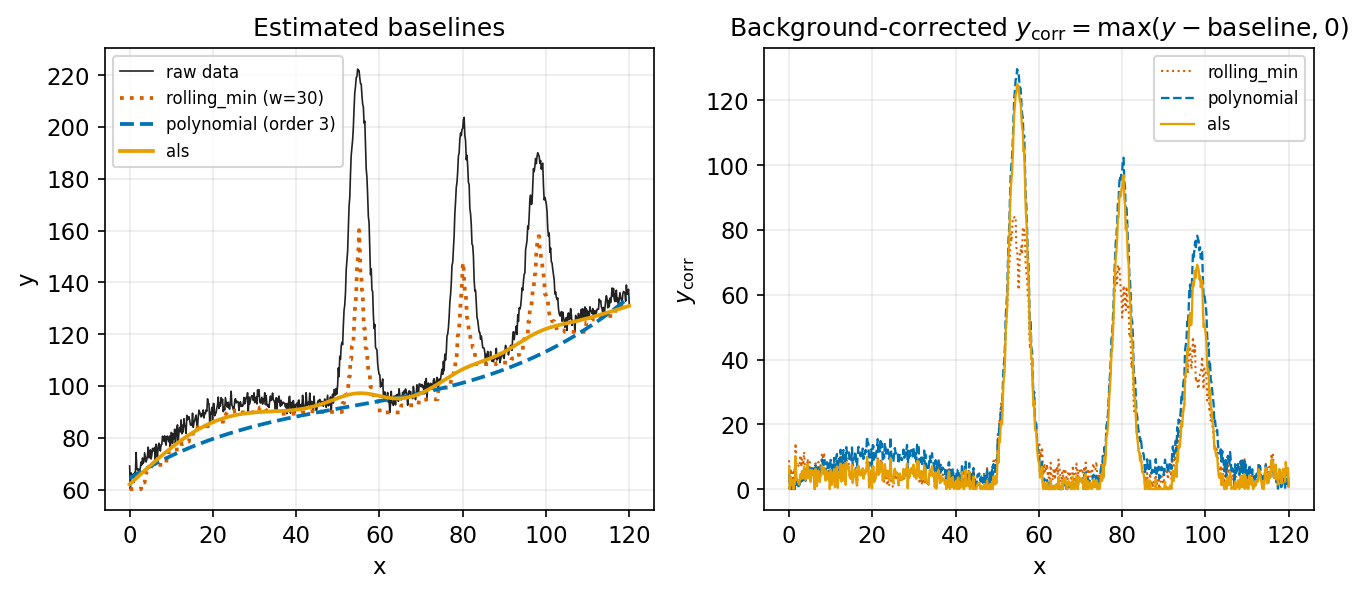
\includegraphics[width=\linewidth]{figures/fig_baselines.png}
\caption{Die drei Basislinien-Methoden auf einem gekr\"ummten, verrauschten
Untergrund. Links: die gesch\"atzten Basislinien --- das rollende Minimum folgt der
unteren Einh\"ullenden in Stufen, Polynom und ALS sind glatt. Rechts: das
korrigierte Signal; ALS und das Polynom ebnen den Untergrund zwischen den Peaks
sauberer ein.}
\label{fig:baselines}
\end{figure}

\paragraph{Die vier Such-Slider.} Die automatische Suche
(\code{scipy.signal.find_peaks} auf dem untergrundkorrigierten Signal) wird von
vier Reglern gesteuert, die in der GUI live wirken:
\begin{itemize}
\item \textbf{Prominenz} (\code{prominence_init}, y-Einheiten): wie weit ein
  Peak aus seiner lokalen Umgebung herausragen muss --- die H\"ohe des Gipfels
  \"uber dem h\"oheren der beiden benachbarten T\"aler, nicht der absolute
  y-Wert. Das ist der wichtigste Regler gegen Rauschen: erh\"ohen, um
  Rauschspitzen zu verwerfen, senken, um schwache Banden zu fangen.
\item \textbf{Mindestabstand} (\code{distance_init}, in Datenpunkten): der
  kleinste erlaubte Abstand zwischen zwei gefundenen Peaks. Verhindert, dass
  eine verrauschte Flanke als mehrere dicht stehende Peaks gez\"ahlt wird;
  liegen zwei Kandidaten n\"aher zusammen, gewinnt der prominentere.
\item \textbf{Mindest-SNR} (\code{min_snr_init}): ein Kandidat wird nur
  akzeptiert, wenn seine H\"ohe mindestens das \code{min_snr_init}-fache des
  gesch\"atzten Rauschens betr\"agt. Erg\"anzt die Prominenz um ein
  rauschbezogenes Kriterium.
\item \textbf{Untergrundfenster} (\code{bg_window}, in Punkten): die Fenster\-breite
  der Untergrundsch\"atzung (rollendes Minimum bzw.\ die gew\"ahlte
  \code{baseline_method}), die \emph{vor} der Suche abgezogen wird. Zu klein
  frisst echte Peaks an, zu gro\ss\ l\"asst eine gekr\"ummte Basislinie stehen;
  $0$ schaltet den Abzug ab. Derselbe Untergrund geht in den Fit und die
  Pr\"asenzpr\"ufung ein.
\end{itemize}
In der GUI kann man die Peaks auch einfach anklicken (Linksklick setzen,
Rechtsklick entfernen), was oft schneller ist als das Feinjustieren der Regler.

\paragraph{Toleranz (\code{tolerance}).} Das $\pm$-Fenster, in dem ein
Komponenten-Peak als ,,derselbe`` wie ein Referenz-Peak gilt. Gr\"o\ss er als die
typische Schwerpunktsverschiebung zwischen Spektren w\"ahlen, aber kleiner als der
Peak-Abstand.

\paragraph{Positionsverfeinerung (\code{refine}).} Standardm\"a\ss ig aus.
Aktivieren, wenn die Positionen leicht daneben liegen (z.\,B.\ eine kleine
Kalibrierverschiebung): die Zentren werden dann innerhalb von \code{refine_window}
verfeinert, w\"ahrend die Amplituden nichtnegativ bleiben
(Abbildung~\ref{fig:refine}). Aus lassen, wenn die Positionen bekannt und
verl\"asslich sind.

\begin{figure}[h]\centering
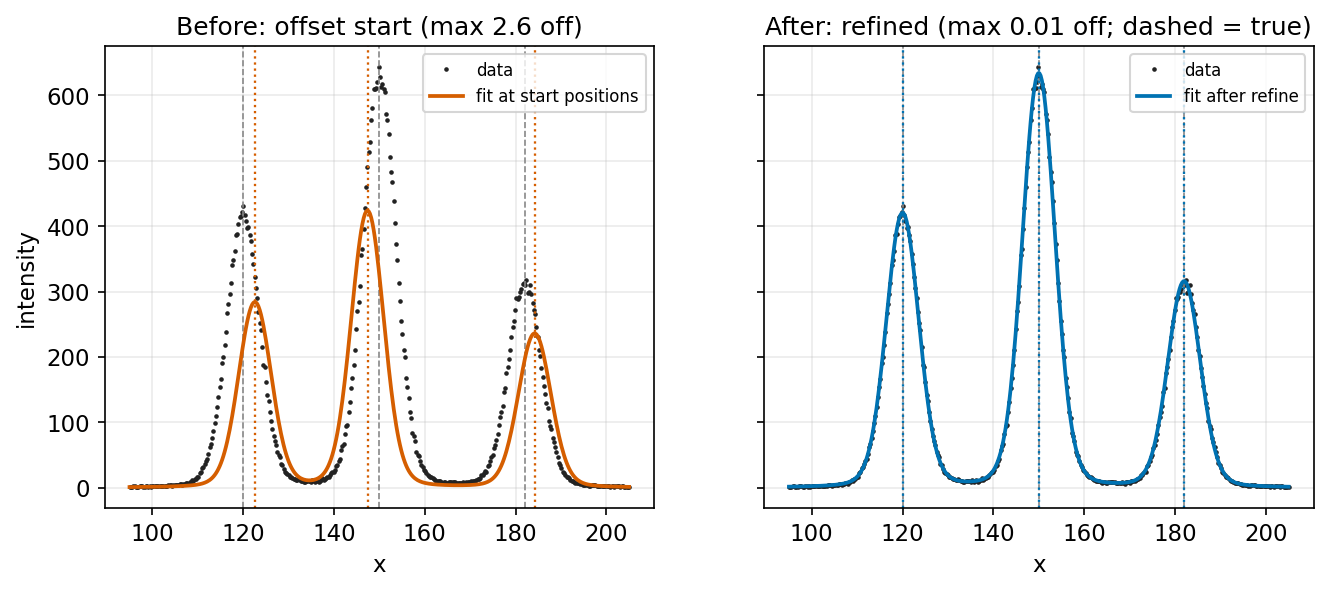
\includegraphics[width=\linewidth]{figures/fig_refine.png}
\caption{Optionale Positionsverfeinerung. Links: ein Fit mit absichtlich
versetzten Startpositionen (gepunktet) verfehlt die wahren Zentren (grau
gestrichelt). Rechts: mit \code{refine = true} werden die Zentren bis auf einen
kleinen Bruchteil eines Punktes zur\"uckgewonnen.}
\label{fig:refine}
\end{figure}

\paragraph{Breitenverfeinerung (\code{refine_widths}).} Standardm\"a\ss ig aus;
sonst bleiben die Breiten f\"ur alle Peaks auf der instrumentellen Aufl\"osung.
Aktivieren, wenn eine Bande wirklich breiter als das Instrument ist (z.\,B.\
unaufgel\"oste Aufspaltung oder inhomogene Verbreiterung). Dann wird eine Breite
pro Peak verfeinert, beschr\"ankt zwischen \code{width_min_factor} und
\code{width_max_factor} mal der instrumentellen Breite; \code{width_mode} w\"ahlt,
ob der ganze Voigt (\code{"fwhm"}) oder nur der Gau\ss-Anteil (\code{"sigma"})
breiter wird (Abbildung~\ref{fig:widths}). Die Obergrenze eng halten: zus\"atzliche
freie Breiten senken das reduzierte $\chi^2_\nu$ immer, und bei \"uberlappenden
oder schwachen Peaks tauschen Breite und Amplitude --- ein kleineres $\chi^2_\nu$
ist also f\"ur sich genommen kein Beleg f\"ur ein besseres Modell.

\begin{figure}[h]\centering
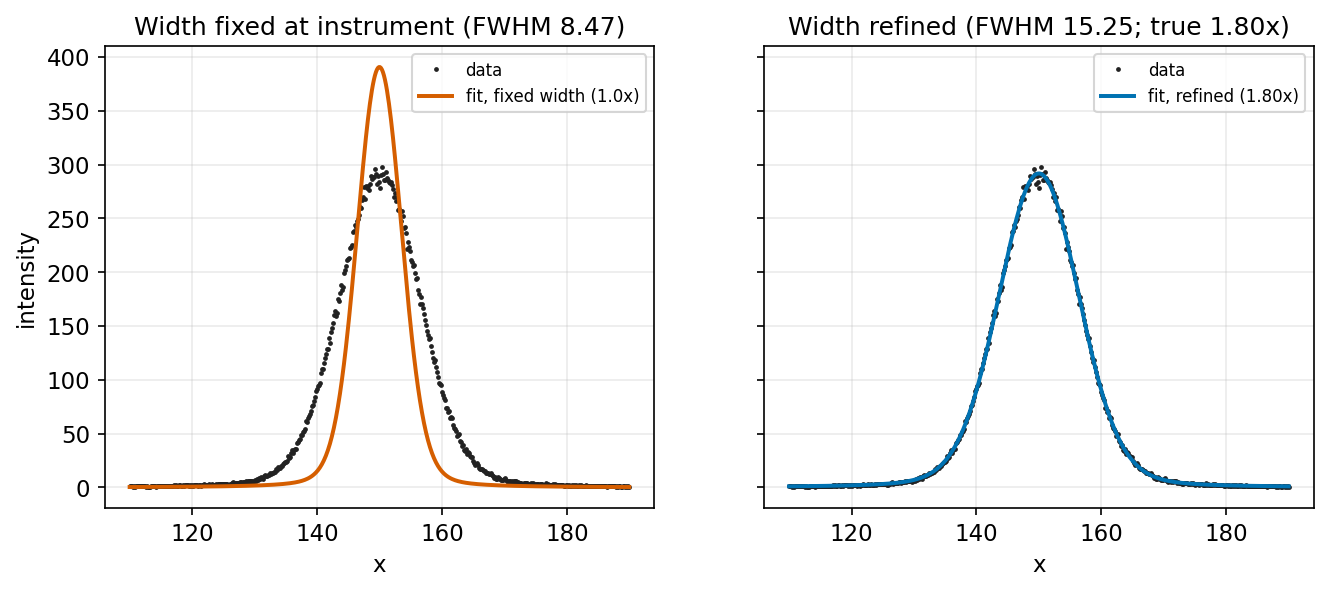
\includegraphics[width=\linewidth]{figures/fig_widths.png}
\caption{Optionale Breitenverfeinerung an einem Peak, der wirklich breiter als das
Instrument ist. Links: mit fester instrumenteller Breite erreicht der Fit die
Daten nicht. Rechts: mit \code{refine_widths = true} wird die eine Breite pro Peak
zur\"uckgewonnen (hier ein Faktor nahe der wahren Verbreiterung), begrenzt durch
\code{width_min_factor}\,..\,\code{width_max_factor}.}
\label{fig:widths}
\end{figure}

% =====================================================================
\section{Ausgabedateien}
Alle Ergebnisse werden neben der Referenzdatei abgelegt; ein etwaiger Suchbereich
erscheint im Dateinamen (z.\,B.\ \code{_90_200}).

\begin{table}[h]\small\centering
\begin{tabularx}{\linewidth}{@{}l L@{}}
\toprule
\textbf{Datei} & \textbf{Inhalt}\\
\midrule
\code{*_fit.png} & Fit mit Einzelkomponenten und Residuenpanel\\
\code{*_peaks.png} & je Komponente eine markierte Abbildung (gr\"un $=$ vorhanden, rot $=$ fehlt)\\
\code{*_results.xlsx} & Excel mit sechs Bl\"attern: Intensities, Positions, Presence, Fit\_Data, Components\_Raw, Parameters (Components\_Raw nur, wenn Komponenten ausgewertet werden)\\
\code{*_results.csv} & eine reine 7-bit-ASCII-CSV mit f\"unf benannten Sektionen (Intensities, Positions, Presence, Fit\_Data, Components\_Raw) und dem vollst\"andigen Parameterblock als Kopfzeile\\
\bottomrule
\end{tabularx}
\end{table}

Das Excel-Blatt \code{Presence} ist die Kernaussage: eine Bin\"armatrix, die f\"ur
jeden Peak und jede Komponente $1$ (gr\"un, vorhanden) oder $0$ (rot, fehlt)
zeigt. Das Blatt \code{Parameters} dokumentiert jeden Lauf vollst\"andig, sodass
er reproduzierbar bleibt.

\paragraph{Die Plots lesen.} Abbildungen~\ref{fig:fit_annot} und
\ref{fig:presence_annot} beschriften die beiden Plottypen. Im Fit-Plot ist die
schwarze Kurve die Summe, die farbigen Kurven sind die einzelnen Peaks (jede
Fl\"ache ist die gefittete Amplitude), und das untere Feld zeigt die Residuen ---
ein guter Fit l\"asst sie strukturlos um null streuen, und der Titel nennt
$\chi^2_\nu$, $R^2$ und die Zahl der aktiven Peaks. In einem Komponenten-Plot
bedeutet eine gr\"une gestrichelte Linie mit Marker, dass der Peak vorhanden ist
($1$); eine rote Linie bedeutet abwesend ($0$). Die Entscheidung f\"allt innerhalb
des $\pm$\code{tolerance}-Fensters (schattiert) anhand der SNR-Schwelle.

\begin{figure}[h]\centering
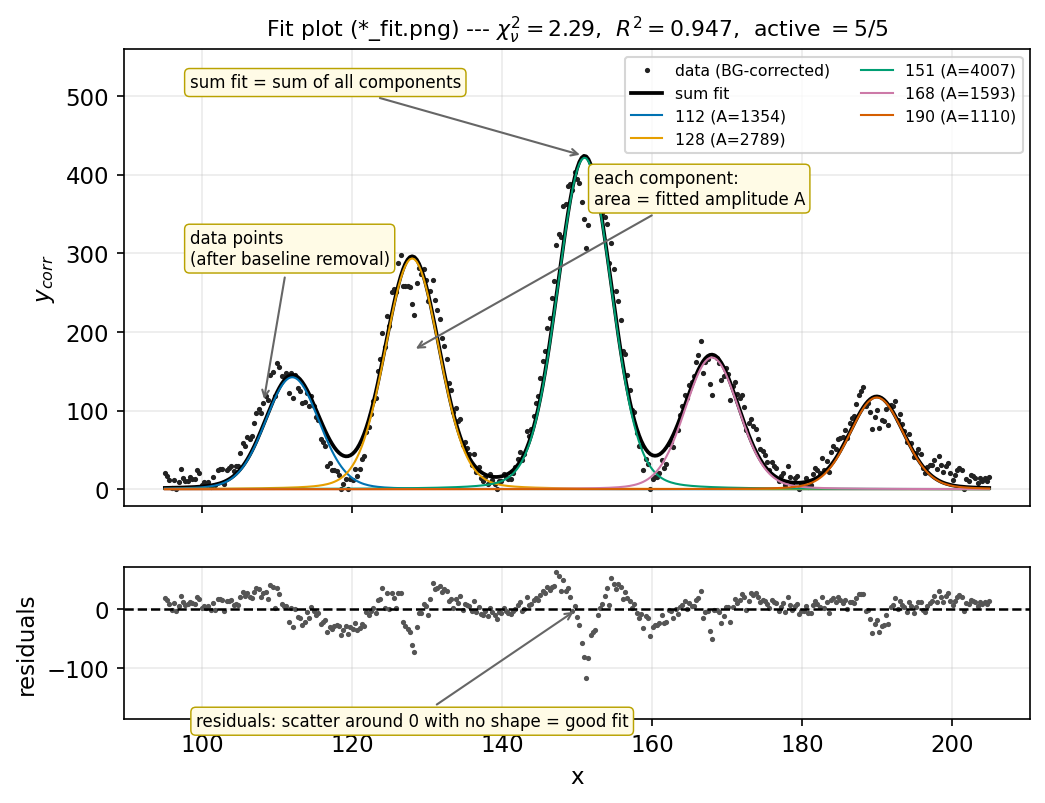
\includegraphics[width=0.92\linewidth]{figures/fig_fit_annotated.png}
\caption{So liest man \code{*_fit.png}: die Daten nach Untergrundabzug, der
summierte Fit, die einzelnen Komponenten (Fl\"ache $=$ Amplitude), die
G\"utezusammenfassung im Titel und das Residuenfeld darunter.}
\label{fig:fit_annot}
\end{figure}

\begin{figure}[h]\centering
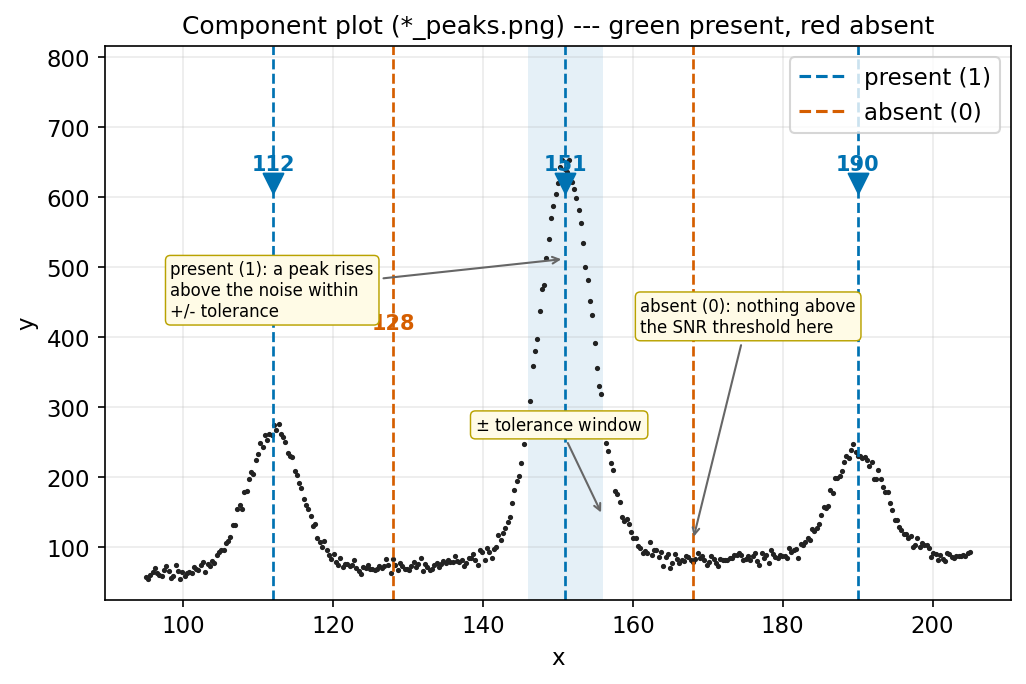
\includegraphics[width=0.92\linewidth]{figures/fig_presence_annotated.png}
\caption{So liest man \code{*_peaks.png}: ein gr\"uner Marker/eine gr\"une Linie
markiert einen vorhandenen Peak ($1$), eine rote Linie einen abwesenden ($0$); die
Entscheidung f\"allt innerhalb des $\pm$\code{tolerance}-Fensters (schattiert).}
\label{fig:presence_annot}
\end{figure}

\bigskip
% =====================================================================
\section{Fehlerbehebung \& FAQ}
\begin{description}
\item[Die GUI startet nicht.] Auf einem Rechner ohne Display oder ohne Tk die
Kommandozeile nutzen: \code{peakcheck --config job.toml --no-gui}. Unter
Debian/Ubuntu Tk per \code{sudo apt install python3-tk} installieren.
\item[\textnormal{,,\code{--no-gui needs a config file}``.}] Der Headless-Modus
braucht eine TOML (oder zumindest \code{--reference}). Eine Vorlage schreiben mit
\code{peakcheck --write-template job.toml}.
\item[Es werden keine Peaks gefunden.] \code{prominence_init} und/oder
\code{min_snr_init} senken, das Suchfenster \code{x_min}/\code{x_max} pr\"ufen oder
die Peaks in der GUI anklicken. Die \emph{x conversion} pr\"ufen, damit die
Positionen in den erwarteten Einheiten liegen.
\item[Reduziertes $\chi^2_\nu$ liegt weit \"uber 1.] Das Modell mit fester Form wird
strapaziert: die Breiten \code{wg}/\code{wl} passen vermutlich nicht zu den Daten,
oder ein Peak fehlt. Fehlenden Peak erg\"anzen oder Breiten korrigieren; die
Amplituden bleiben der beste nichtnegative Fit.
\item[Gesetzte Peaks verschwinden nach dem Fit (aktive Anzahl sinkt) oder der Fit
ist ein breiter Hügel.] Das Profil ist viel breiter als die Peaks der Daten; die
\"uberlappenden Profile werden redundant, und der nichtnegative Fit setzt einige
Amplituden auf null. Fast immer sind \code{wg}/\code{wl} auf der falschen Skala:
z.\,B.\ instrumentelle Werte in cm\textsuperscript{-1}, w\"ahrend die Daten noch in
meV vorliegen, weil die \emph{x-Umrechnung} aus ist. Umrechnung setzen (oder die
passende Config laden) oder \code{wg}/\code{wl} grob auf die Halbwertsbreite der
Peaks stellen. PeakCheck gibt in diesem Fall einen Hinweis aus. Die Marker- und
die Fit-Beschriftung zeigen stets dieselben Positionen; nur ihre angezeigte
Genauigkeit stimmt jetzt \"uberein (eine Nachkommastelle), ein Peak ,,wandert`` also
nicht zwischen Setzen und Fitten.
\item[Ein erwarteter Peak gilt als ,,abwesend``.] \code{tolerance} erh\"ohen, wenn
der Komponenten-Peak verschoben ist, oder \code{snr_thresh} f\"ur eine verrauschte
Komponente senken. Pr\"ufen, ob \code{presence_baseline_corrected} der Absicht
entspricht (H\"ohe \"uber Basislinie vs.\ Rohsignal).
\item[Die gemeldeten Fehler wirken falsch.] Mit echter Fehlerspalte liefert der
Modus \code{statistical} wahre $1\sigma$; ohne sie werden Fehler mit
$\sqrt{\chi^2_\nu}$ skaliert. F\"ur Z\"ahldaten \"uber viele Gr\"o\ss enordnungen eine
Fehlerspalte angeben. Das Supplement zeigt eine Monte-Carlo-Pr\"ufung des
Fehlerbudgets.
\item[Die Datei l\"adt nicht.] PeakCheck liest zwei- oder dreispaltigen
Whitespace- oder CSV-Text und ignoriert Kommentarzeilen, die mit \texttt{\#},
\texttt{!} oder \texttt{\%} beginnen; nicht-finite Zeilen werden verworfen.
Trennzeichen und Fehlerspalten-Einstellung pr\"ufen.
\item[Kann ich einen Lauf exakt reproduzieren?] Ja --- die Config speichern
(\emph{Save config}, Strg+S) oder den Parameterblock aus dem CSV-Kopf bzw.\ dem
Excel-Blatt \code{Parameters} wiederverwenden und mit \code{--config} erneut
ausf\"uhren.
\end{description}

\noindent\rule{\linewidth}{0.4pt}\\[2pt]
{\footnotesize PeakCheck \textperiodcentered\ Anleitung \textperiodcentered\
\textcopyright\ 2026 Lukas Knauer, RPTU Kaiserslautern-Landau, AG Sch\"unemann
\textperiodcentered\ Die technischen Details aller Rechenschritte stehen im
begleitenden Supplement.}

\end{document}
